
\chapter{Introduction to industrial instrumentation}

Instrumentation is the science of automated measurement and control.  Applications of this science abound in modern research, industry, and everyday living.  From automobile engine control systems to home thermostats to aircraft autopilots to the manufacture of pharmaceutical drugs, automation surrounds us.  This chapter explains some of the fundamental principles of industrial instrumentation.
 
\vskip 10pt

The first step, naturally, is measurement.  If we can't measure something, it is really pointless to try to control it.  This ``something'' usually takes one of the following forms in industry:

\begin{itemize}
\item Fluid pressure
\item Fluid flow rate
\item The temperature of an object
\item Fluid volume stored in a vessel
\item Chemical concentration
\item Machine position, motion, or acceleration
\item Physical dimension(s) of an object
\item Count (inventory) of objects
\item Electrical voltage, current, or resistance
\end{itemize}

Once we measure the quantity we are interested in, we usually transmit a signal representing this quantity to an indicating or computing device where either human or automated action then takes place.  If the controlling action is automated, the computer sends a signal to a final controlling device which then influences the quantity being measured.  

\filbreak

This final control device usually takes one of the following forms:

\begin{itemize}
\item Control valve (for throttling the flow rate of a fluid)
\item Electric motor
\item Electric heater
\end{itemize}

Both the measurement device and the final control device connect to some physical system which we call the \textit{process}.  To show this as a general block diagram:

$$\includegraphics{intro_00.eps}$$

The common home thermostat is an example of a measurement and control system, with the home's internal air temperature being the ``process'' under control.  In this example, the thermostat usually serves two functions: sensing and control, while the home's heater adds heat to the home to increase temperature, and/or the home's air conditioner extracts heat from the home to decrease temperature.  The job of this control system is to maintain air temperature at some comfortable level, with the heater or air conditioner taking action to correct temperature if it strays too far from the desired value (called the \textit{setpoint}).

\vskip 10pt

Industrial measurement and control systems have their own unique terms and standards, which is the primary focus of this lesson.  Here are some common instrumentation terms and their definitions:

\vskip 10pt

\noindent
\textbf{Process}: The physical system we are attempting to control or measure.  \textit{Examples: water filtration system, molten metal casting system, steam boiler, oil refinery unit, power generation unit.} \index{Process}

\vskip 10pt

\noindent
\textbf{Process Variable}, or \textbf{PV}: The specific quantity we are measuring in a process.  \textit{Examples: pressure, level, temperature, flow, electrical conductivity, pH, position, speed, vibration.} \index{Process variable}

\vskip 10pt

\noindent
\textbf{Setpoint}, or \textbf{SP}: The value at which we desire the process variable to be maintained at.  In other words, the ``target'' value for the process variable. \index{Setpoint}

\vskip 10pt

\noindent
\textbf{Primary Sensing Element}, or \textbf{PSE}: A device directly sensing the process variable and translating that sensed quantity into an analog representation (electrical voltage, current, resistance; mechanical force, motion, etc.).  \textit{Examples: thermocouple, thermistor, bourdon tube, microphone, potentiometer, electrochemical cell, accelerometer.} \index{Primary sensing element}

\vskip 10pt

\noindent
\textbf{Transducer}: A device converting one standardized instrumentation signal into another standardized instrumentation signal, and/or performing some sort of processing on that signal.  Often referred to as a \textit{converter} and sometimes as a ``relay.''  \textit{Examples: I/P converter (converts 4-20 mA electric signal into 3-15 PSI pneumatic signal), P/I converter (converts 3-15 PSI pneumatic signal into 4-20 mA electric signal), square-root extractor (calculates the square root of the input signal).} \index{Transducer}  \index{Converter}  \index{Relay}

Note: in general science parlance, a ``transducer'' is any device converting one form of energy into another, such as a microphone or a thermocouple.  In industrial instrumentation, however, we generally use ``primary sensing element'' to describe this concept and reserve the word ``transducer'' to specifically refer to a conversion device for standardized instrumentation signals.

\vskip 10pt

\noindent
\textbf{Transmitter}: A device translating the signal produced by a primary sensing element (PSE) into a \textit{standardized} instrumentation signal such as 3-15 PSI air pressure, 4-20 mA DC electric current, Fieldbus digital signal packet, etc., which may then be conveyed to an indicating device, a controlling device, or both. \index{Transmitter}

\vskip 10pt

\noindent
\textbf{Lower- and Upper-range values}, abbreviated \textbf{LRV} and \textbf{URV}, respectively: the values of process measurement deemed to be 0\% and 100\% of a transmitter's calibrated range.  For example, if a temperature transmitter is calibrated to measure a range of temperature starting at 300 degrees Celsius and ending at 500 degrees Celsius, its LRV would be 300 $^{o}$C and its URV would be 500 $^{o}$C. \index{LRV} \index{URV} \index{Lower range value} \index{Upper range value}

\vskip 10pt

\noindent
\textbf{Zero} and \textbf{Span}: alternative descriptions to LRV and URV for the 0\% and 100\% points of an instrument's calibrated range.  ``Zero'' refers to the beginning-point of an instrument's range (equivalent to LRV), while ``span'' refers to the width of its range (URV $-$ LRV).  For example, if a temperature transmitter is calibrated to measure a range of temperature starting at 300 degrees Celsius and ending at 500 degrees Celsius, its zero would be 300 $^{o}$C and its span would be 200 $^{o}$C.  \index{Zero} \index{Span}

\vskip 10pt

\noindent
\textbf{Controller}: A device receiving a process variable (PV) signal from a primary sensing element (PSE) or transmitter, comparing that signal to the desired value (called the setpoint) for that process variable, and calculating an appropriate output signal value to be sent to a final control element (FCE) such as an electric motor or control valve.  \index{Controller}

\vskip 10pt

\noindent
\textbf{Final Control Element}, or \textbf{FCE}: A device receiving the signal output by a controller to directly influence the process.  \textit{Examples: variable-speed electric motor, control valve, electric heater.} \index{Final Control Element}

\vskip 10pt

\noindent
\textbf{Manipulated Variable}, or \textbf{MV}: The quantity in a process we adjust or otherwise manipulate in order to influence the process variable (PV).  Also used to describe the output signal generated by a controller; i.e. the signal commanding (``manipulating'') the final control element to influence the process. \index{Manipulated variable}  \index{MV}

\vskip 10pt

\noindent
\textbf{Automatic mode}: When the controller generates an output signal based on the relationship of process variable (PV) to the setpoint (SP). \index{Automatic mode}  

\vskip 10pt

\noindent
\textbf{Manual mode}: When the controller's decision-making ability is bypassed to let a human operator directly determine the output signal sent to the final control element. \index{Manual mode}

\vskip 20pt

Now we will explore some practical examples of measurement and control systems so you can get a better idea of these fundamental concepts.








\filbreak
\section{Example: boiler water level control system} 
 
Steam boilers are very common in industry, principally because steam power is so useful.  Common uses for steam in industry include doing mechanical work (e.g. a steam engine moving some sort of machine), heating, producing vacuums (through the use of ``steam ejectors''), and augmenting chemical processes (e.g. reforming of natural gas into hydrogen and carbon dioxide).  

The process of converting water into steam is quite simple: heat up the water until it boils.  Anyone who has ever boiled a pot of water for cooking knows how this process works.  Making steam continuously, however, is a little more complicated.  An important variable to measure and control in a continuous boiler is the level of water in the ``steam drum'' (the upper vessel in a water-tube boiler).  In order to safely and efficiently produce a continuous flow of steam, we must ensure the steam drum never runs too low on water, or too high.  If there is not enough water in the drum, the water tubes may run dry and burn through from the heat of the fire.  If there is too much water in the drum, liquid water may be carried along with the flow of steam, causing problems downstream.

\filbreak

In this next illustration, you can see the essential elements of a water level control system, showing transmitter, controller, and control valve:

$$\includegraphics{intro_01.eps}$$

The first instrument in this control system is the \textit{level transmitter}, or ``LT''.  The purpose of this device is to sense the water level in the steam drum and report (``transmit'') that measurement to the controller in the form of a signal.  In this case, the type of signal is \textit{pneumatic}: a variable air pressure sent through metal or plastic tubes.  The greater the water level in the drum, the more air pressure output by the level transmitter.  Since the transmitter is pneumatic, it must be supplied with a source of clean, compressed air on which to operate.  This is the meaning of the ``A.S.'' tube (Air Supply) entering the top of the transmitter.

This pneumatic signal is sent to the next instrument in the control system, the \textit{level indicating controller}, or ``LIC''.  The purpose of this instrument is to compare the level transmitter's signal against a \textit{setpoint} value entered by a human operator representing the desired water level in the steam drum.  The controller then generates an \textit{output} signal telling the control valve to either introduce more or less water into the boiler to maintain the steam drum water level at setpoint.  As with the transmitter, the controller in this system is pneumatic, operating entirely on compressed air.  This means the output of the controller is also a variable air pressure signal, just like the signal output by the level transmitter.  Naturally, the controller requires a constant supply of clean, compressed air on which to run, which explains the ``A.S.'' (Air Supply) tube connecting to it.
 
The last instrument in this control system is the control valve, operated directly by the air pressure signal output by the controller.  Its purpose is to influence the flow rate of water into the boiler, ``throttling'' the water flow more or less as determined by controller.  This particular type of control valve uses a large diaphragm and a large spring to move the valve further open with more signal pressure and further closed with less signal pressure.

\vskip 10pt

When the controller is placed in the ``automatic'' mode, it will move the control valve to whatever position necessary to maintain a constant steam drum water level.  The phrase ``whatever position necessary'' suggests the relationship between the controller output signal, the process variable signal (PV), and the setpoint (SP) is complex.  If the controller senses a water level above setpoint, it will close off the valve as far as necessary to decrease the water level down to setpoint.  Conversely, if the controller senses a water level below setpoint, it will open up the valve as far as necessary to raise the water level up to setpoint.  

What this means in a practical sense is that the controller's output signal (equating to valve position) in automatic mode is just as much a function of process load (i.e. how much steam is being used from the boiler) as it is a function of setpoint (i.e. where we wish the water level to be).  Consider a situation where the steam demand from the boiler is very low.  If there isn't much steam being drawn off the boiler, this means there will be little water boiled into steam and therefore little need for additional feedwater to be pumped into the boiler.  Therefore, in this situation, one would expect the control valve to hover near the fully-closed position, allowing just enough water into the boiler to keep the steam drum water level at setpoint.  If, however, there is a high demand for steam from this boiler, the rate of evaporation will be much greater.  This means the control system must add feedwater to the boiler at a much greater flow rate in order to maintain the steam drum water level at setpoint.  In this situation we would expect to see the control valve much closer to being fully-open as the control system ``works harder'' to maintain a constant water level in the steam drum.  Thus, we see how the controller automatically positions the control valve to react to different boiler operating conditions even when the setpoint is fixed.

\vskip 10pt

A human operator supervising this boiler has the option of placing the controller into ``manual'' mode.  In this mode the control valve position is under direct control of the human operator, with the controller essentially ignoring the signal sent from the water level transmitter.  Being an indicating controller, the controller faceplate will still show how much water is in the steam drum, but it is now the human operator's sole responsibility to move the control valve to the appropriate position to hold water level at setpoint -- \textit{in manual mode the controller takes no corrective action of its own}.  Manual mode is useful to human operators during start-up and shut-down conditions.  It is also useful to instrument technicians for troubleshooting misbehaving control systems.  Placing a controller into manual mode is akin to disengaging the cruise control in an automobile, transferring control of engine power from the car's computer back to the human driver.  One can easily imagine an automobile mechanic needing to throttle a car's engine ``manually'' (i.e. with the cruise control turned off) in order to properly diagnose an engine or drivetrain problem.  This is true for industrial processes as well, where instrument technicians may need to place a controller into manual mode in order to properly diagnose transmitter or control valve problems.

\vskip 10pt

\filbreak

As was mentioned before, this is an example of a \textit{pneumatic} (compressed air) control system, where all the instruments operate on compressed air, and use compressed air as the signaling medium.  Pneumatic instrumentation is an old technology, dating back to the early twentieth century.  While most modern instruments are electronic in nature, pneumatic instruments still find application within industry.  The most common industry standard for pneumatic pressure signals is 3 to 15 PSI, with 3 PSI representing low end-of-scale and 15 PSI representing high end-of-scale.  Alternative pressure ranges for pneumatic signals sometimes encountered in industry include 3 to 27 PSI, and 6 to 30 PSI.  The following table shows the relationship between air signal pressure and steam drum level for this boiler's 3-15 PSI level transmitter: \index{Pneumatic control system}

% No blank lines allowed between lines of an \halign structure!
% I use comments (%) instead, so Tex doesn't choke.

$$\vbox{\offinterlineskip
\halign{\strut
\vrule \quad\hfil # \ \hfil & 
\vrule \quad\hfil # \ \hfil \vrule \cr
\noalign{\hrule}
%
% First row
\textbf{Transmitter air signal pressure} & \textbf{Steam drum water level} \cr
%
\noalign{\hrule}
%
% Another row
3 PSI & 0\% (Empty) \cr
%
\noalign{\hrule}
%
% Another row
6 PSI & 25\% \cr
%
\noalign{\hrule}
%
% Another row
9 PSI & 50\%  \cr
%
\noalign{\hrule}
%
% Another row
12 PSI & 75\% \cr
%
\noalign{\hrule}
%
% Another row
15 PSI & 100\% (Full) \cr
%
\noalign{\hrule}
} % End of \halign 
}$$ % End of \vbox

It should be noted this table assumes the transmitter measures the \textit{full range} of water level possible in the drum.  Usually, this is not the case.  Instead, the transmitter will be calibrated so it only senses a narrow range of water level near the middle of the drum.  Thus, 3 PSI (0\%) will not represent an empty drum, and neither will 15 PSI (100\%) represent a completely full drum.  Calibrating the transmitter like this helps avoid the possibility of actually running the drum completely empty or completely full in the case of an operator incorrectly setting the setpoint value near either extreme end of the measurement scale.

An example table showing this kind of realistic transmitter calibration appears here:

% No blank lines allowed between lines of an \halign structure!
% I use comments (%) instead, so Tex doesn't choke.

$$\vbox{\offinterlineskip
\halign{\strut
\vrule \quad\hfil # \ \hfil & 
\vrule \quad\hfil # \ \hfil \vrule \cr
\noalign{\hrule}
%
% First row
\textbf{Transmitter air signal pressure} & \textbf{Actual steam drum water level} \cr
%
\noalign{\hrule}
%
% Another row
3 PSI & 40\% \cr
%
\noalign{\hrule}
%
% Another row
6 PSI & 45\% \cr
%
\noalign{\hrule}
%
% Another row
9 PSI & 50\%  \cr
%
\noalign{\hrule}
%
% Another row
12 PSI & 55\% \cr
%
\noalign{\hrule}
%
% Another row
15 PSI & 60\% \cr
%
\noalign{\hrule}
} % End of \halign 
}$$ % End of \vbox

\vskip 10pt

\filbreak

The boiler's steam drum level controller outputs a pneumatic output signal to the control valve, using the same 3 to 15 PSI standard to command different valve positions:

% No blank lines allowed between lines of an \halign structure!
% I use comments (%) instead, so Tex doesn't choke.

$$\vbox{\offinterlineskip
\halign{\strut
\vrule \quad\hfil # \ \hfil & 
\vrule \quad\hfil # \ \hfil \vrule \cr
\noalign{\hrule}
%
% First row
\textbf{Controller output signal pressure} & \textbf{Control valve position} \cr
%
\noalign{\hrule}
%
% Another row
3 PSI & 0\% open (Fully shut) \cr
%
\noalign{\hrule}
%
% Another row
6 PSI & 25\% open \cr
%
\noalign{\hrule}
%
% Another row
9 PSI & 50\% open \cr
%
\noalign{\hrule}
%
% Another row
12 PSI & 75\% open \cr
%
\noalign{\hrule}
%
% Another row
15 PSI & 100\% (Fully open) \cr
%
\noalign{\hrule}
} % End of \halign 
}$$ % End of \vbox

Even though the same range of air pressure (3 to 15 PSI) is used to represent water level in the steam drum \textit{and} the position of the control valve, there is no simple correspondence between the two signals.  A common misconception for students new to this topic is to assume the transmitter signal (PV) and controller output signal must be identical.  \textit{This is not true}.  Typically the 3-15 PSI signal representing level will be at some value different from the 3-15 PSI signal driving the valve, because those two signals represent two entirely different variables in the boiler system.  As we have seen previously, the output signal from a controller in automatic mode is just as much a function of process conditions as it is a function of the measured variable.  This error is akin to thinking the road speed signal in an automobile cruise control system (the ``process variable'' or PV) must be the same value as the signal sent by the cruise control computer to the engine's accelerator control (the controller's ``output'' signal).  Granted, these two signals are \textit{related} to one another, but since they represent two different parameters in the controlled system we have no reason to expect their values will be \textit{equal} except by chance.





\filbreak
\section{Example: wastewater disinfection} 

The final step in treating wastewater before releasing it into the natural environment is to kill any harmful microorganisms (e.g. viruses, bacteria) in it.  This is called \textit{disinfection}, and chlorine gas is a very effective disinfecting agent.  However, just as it is not good to mix too little chlorine in the outgoing water (effluent) because we might not disinfect the water thoroughly enough, there is also danger of injecting too much chlorine in the effluent because then we might begin poisoning animals and beneficial microorganisms in the natural environment. \index{Wastewater disinfection}

To ensure the right amount of chlorine injection, we must use a dissolved chlorine analyzer to measure the chlorine concentration in the effluent, and use a controller to automatically adjust the chlorine control valve to inject the right amount of chlorine at all times.  The following P\&ID (Process and Instrument Diagram) shows how such a control system might look:

$$\includegraphics{intro_02.eps}$$

Chlorine gas coming through the control valve mixes with the incoming water (influent), then has time to disinfect in the contact chamber before exiting out to the environment.

The transmitter is labeled ``AT'' (Analytical Transmitter) because its function is to \textit{analyze} the concentration of chlorine dissolved in the water and \textit{transmit} this information to the control system.  The ``Cl$_{2}$'' (chemical notation for a chlorine molecule) written near the transmitter bubble declares this to be a chlorine analyzer.  The dashed line coming out of the transmitter tells us the signal is electric in nature, not pneumatic as was the case in the previous (boiler control system) example.  The most common and likely standard for electronic signaling in industry is 4 to 20 milliamps DC, which represents chlorine concentration in much the same way as the 3 to 15 PSI pneumatic signal standard represented steam drum water level in the boiler:

$$\vbox{\offinterlineskip
\halign{\strut
\vrule \quad\hfil # \ \hfil & 
\vrule \quad\hfil # \ \hfil \vrule \cr
\noalign{\hrule}
%
% First row
\textbf{Transmitter signal current} & \textbf{Chlorine concentration} \cr
%
\noalign{\hrule}
%
% Another row
4 mA & 0\% (no chlorine) \cr
%
\noalign{\hrule}
%
% Another row
8 mA & 25\% \cr
%
\noalign{\hrule}
%
% Another row
12 mA & 50\%  \cr
%
\noalign{\hrule}
%
% Another row
16 mA & 75\% \cr
%
\noalign{\hrule}
%
% Another row
20 mA & 100\% (Full concentration) \cr
%
\noalign{\hrule}
} % End of \halign 
}$$ % End of \vbox

The controller is labeled ``AIC'' because it is an Analytical Indicating Controller.  Controllers are always designated by the process variable they are charged with controlling, in this case the chlorine analysis of the effluent.  ``Indicating'' means there is some form of display that a human operator or technician can read showing the chlorine concentration.  ``SP'' refers to the setpoint value entered by the operator, which the controller tries to maintain by adjusting the position of the chlorine injection valve.

A dashed line going from the controller to the valve indicates another electronic signal: a 4 to 20 mA direct current signal again.  Just as with the 3 to 15 PSI pneumatic signal standard in the pneumatic boiler control system, the amount of electric current in this signal path directly relates to a certain valve position:

$$\vbox{\offinterlineskip
\halign{\strut
\vrule \quad\hfil # \ \hfil & 
\vrule \quad\hfil # \ \hfil \vrule \cr
\noalign{\hrule}
%
% First row
\textbf{Controller output signal current} & \textbf{Control valve position} \cr
%
\noalign{\hrule}
%
% Another row
4 mA & 0\% open (Fully shut) \cr
%
\noalign{\hrule}
%
% Another row
8 mA & 25\% open \cr
%
\noalign{\hrule}
%
% Another row
12 mA & 50\% open \cr
%
\noalign{\hrule}
%
% Another row
16 mA & 75\% open \cr
%
\noalign{\hrule}
%
% Another row
20 mA & 100\% (Fully open) \cr
%
\noalign{\hrule}
} % End of \halign 
}$$ % End of \vbox

Note: it is possible, and in some cases even preferable, to have either a transmitter or a control valve that responds in reverse fashion to an instrument signal such as 3 to 15 PSI or 4 to 20 milliamps.  For example, this valve could have been set up to be wide open at 4 mA and fully shut at 20 mA.  The main point to recognize here is that both the process variable sensed by the transmitter and the position of the control valve are proportionately represented by analog signals.

Just as with the 3 to 15 PSI pneumatic signals used to represent water level and control valve position in the boiler seen previously, the two 4 to 20 milliamp current signals in this system represent two different variables in the system and therefore will not be equal to each other except by coincidence.  A common misconception for people first learning about analog instrumentation signals is to assume the transmitter's signal (``Process Variable'') must be identical in value to the control valve's signal (``Manipulated Variable'' or ``Output''), but this is not true.

\vskip 10pt

The letter ``M'' inside the control valve bubble tells us this is a motor-actuated valve.  Instead of using compressed air pushing against a spring-loaded diaphragm as was the case in the boiler control system, this valve is actuated by an electric motor turning a gear-reduction mechanism.  The gear reduction mechanism allows slow motion of the control valve stem even though the motor spins at a fast rate.  A special electronic control circuit inside the valve actuator modulates electric power to the electric motor in order to ensure the valve position accurately matches the signal sent by the controller.  In effect, this is another control system in itself, controlling valve position according to a ``setpoint'' signal sent by another device (in this case, the AIT controller which is telling the valve what position to go to).





\filbreak
\section{Example: chemical reactor temperature control} 

Sometimes we encounter a diversity of instrument signal standards in one control system.  Such is the case with the following chemical reactor temperature control system, where three different signal standards convey information between the instruments.  A P\&ID (Process and Instrument Diagram) shows the inter-relationships of the process piping, vessels, and instruments:

$$\includegraphics{intro_03.eps}$$

The purpose of this control system is to ensure the chemical solution inside the reactor vessel is maintained at a constant temperature.  A steam-heated ``jacket'' envelops the reactor vessel, transferring heat from the steam into the chemical solution inside.  The control system maintains a constant temperature by measuring the temperature of the reactor vessel, and throttling steam from a boiler to the steam jacket to add more or less heat as needed. \index{Steam jacket}  \index{Jacket, reactor vessel}

We begin as usual with the temperature transmitter, located near the bottom of the vessel.  Note the different line type used to connect the temperature transmitter (TT) with the temperature-indicating controller (TIC): hollow diamonds with lines in between.  This signifies a \textit{digital electronic instrument signal} -- sometimes referred to as a \textit{fieldbus} -- rather than an analog type (such as 4 to 20 mA or 3 to 15 PSI).  The transmitter in this system is actually a digital computer, and so is the controller.  The transmitter reports the process variable (reactor temperature) to the controller using digital bits of information.  Here there is no analog scale of 4 to 20 milliamps, but rather electric voltage/current pulses representing the 0 and 1 states of binary data. \index{Fieldbus}

Digital instrument signals are capable of transferring multiple data points rather than single data points as is the case with analog instrument signals.  This means digital instrument signals may convey device status information (such as self-diagnostic test results) as well as the basic measurement value.  In other words, the digital signal coming from this transmitter not only tells the controller how hot the reactor is, but it may also communicate to the controller how well the transmitter is functioning.

The dashed line exiting the controller shows it to be analog electronic: most likely 4 to 20 milliamps DC.  This electronic signal does not go directly to the control valve, however.  It passes through a device labeled ``TY'', which is a \textit{transducer} to convert the 4 to 20 mA electronic signal into a 3 to 15 PSI pneumatic signal which then actuates the valve.  In essence, this signal transducer acts as an electrically-controlled air pressure regulator, taking the supply air pressure (usually 20 to 25 PSI) and regulating it down to a level commanded by the controller's electronic output signal.

At the temperature control valve (TV) the 3 to 15 PSI pneumatic pressure signal applies a force on a diaphragm to move the valve mechanism against the restraining force of a large spring.  The construction and operation of this valve is the same as for the feedwater valve in the pneumatic boiler water control system.  The letters ``ATO'' immediately below the valve symbol mean ``Air-To-Open,'' referring to the direction this valve mechanism will move (wider open) as more air signal pressure is applied to its actuator.

\vskip 10pt

A detail not shown on this diagram, yet critically important to the operation of the temperature control system, is the \textit{direction of action} for the controller while in automatic mode.  It is possible to configure general-purpose controllers to act either in a \textit{direct} fashion where an increasing process variable signal automatically results in an increasing output signal, or in a \textit{reverse} fashion where an increasing process variable signal automatically results in a decreasing output signal.  An effective way to identify the proper direction of action for any process controller is to perform a ``thought experiment\footnote{For more information on conducting ``thought experiments,'' refer to the subsection of this book titled ``Using Thought Experiments'' (\ref{using_thought_experiments}) beginning on page \pageref{using_thought_experiments}.}'' whereby we imagine the process variable increasing over time, and then determine which way the controller's output needs to change in order to bring the process variable value back to setpoint based on the final control element's influence within the process.  \index{Thought experiment}  \index{Problem-solving technique: thought experiment}  \index{Direct-acting controller}  \index{Reverse-acting controller}  \index{Action, controller}  \index{Controller action, direct vs. reverse} 

In this process, let us imagine the reactor temperature increasing for some reason, perhaps an increase in the temperature of the feed entering the reactor.  With an increasing temperature, the controller must \textit{reduce} the amount of steam applied to the heating jacket surrounding the reactor in order to correct for this temperature change.  With an air-to-open (ATO) steam valve, this requires a \textit{decreased} air pressure signal to the valve in order to close it further and reduce heat input to the reactor.  Thus, if an increasing process variable signal requires a decreasing controller output signal, the controller in this case needs to be configured for \textit{reverse} action.

We could easily imagine reasons why the temperature controller in this process might have to be configured for direct action instead of reverse action.  If the piping were altered such that the control valve throttled the flow of \textit{coolant} to the reactor rather than steam, an increasing temperature would require a further-open valve, which would only happen if the controller were configured for direct action.  Alternatively, if the steam valve were air-to-close (ATC) rather than air-to-open (ATO), an increasing reactor temperature (requiring less steam be sent to the reactor) would necessitate the controller outputting an increased signal to the valve, so that more air signal pressure pushed the valve further closed.

\vskip 10pt

\filbreak

An example of a chemical reaction temperature control system requiring \textit{direct} controller action is shown in the following photograph.  Here, we see a jacketed stainless-steel vessel used to ferment beer at cold temperatures.  The jacket surrounding this vessel is pumped full of chilled glycol solution (similar to automotive antifreeze), to draw heat away from the fermenting beer and maintain its temperature well below ambient:

$$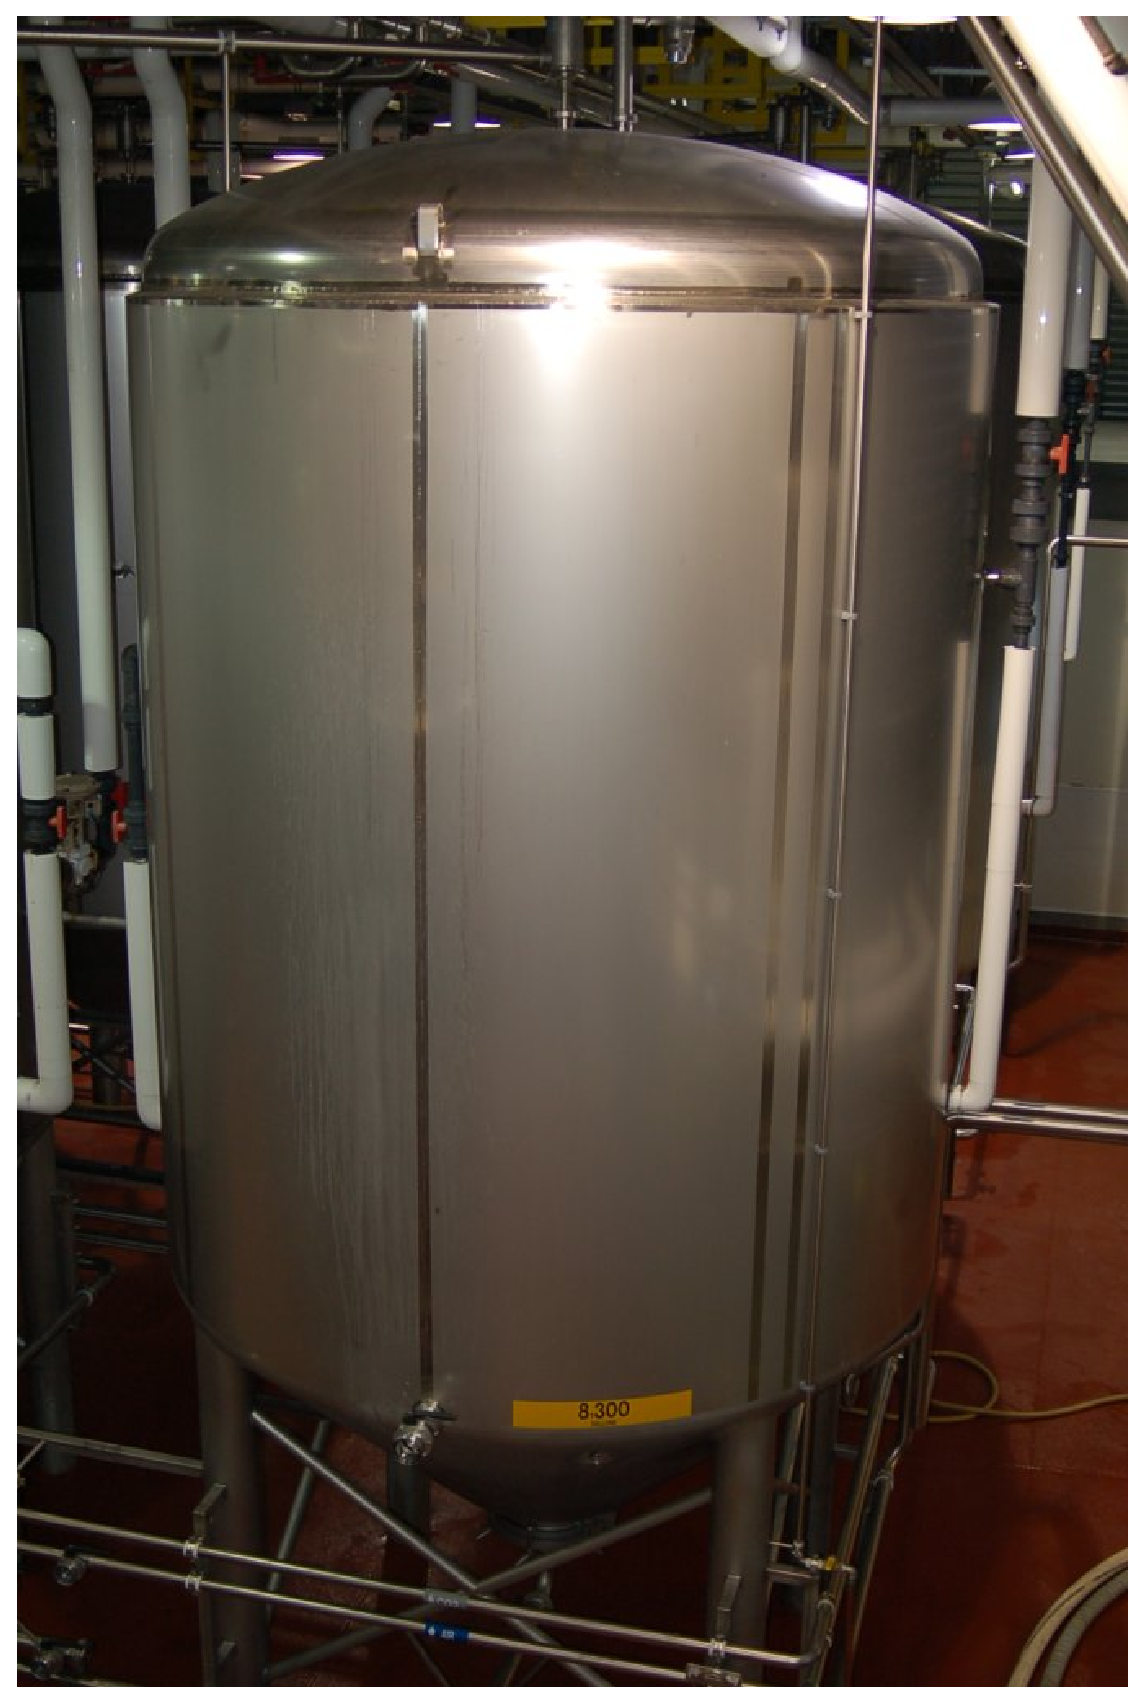
\includegraphics[height=5in]{intro_30.eps}$$

If the beer becomes too warm, the controller sends an increased signal to the glycol valve sending more chilled glycol through the vessel's jacket to remove heat from the beer.  Since the relationship between the controller's process variable and its output is direct (i.e. rising PV results in rising Output), the controller needs to be configured for direct action.

This is why general-purpose process controllers always provide a user-selectable option for either direct or reverse action: it makes them adaptable to the needs of \textit{any} process, no matter the physics of the process or the behavior of the other loop instruments (e.g. transmitter and final control element).

\vskip 10pt

\filbreak

An additional instrument connected to our hypothetical chemical reactor is a pressure transmitter (PT) on the feed line.  While not a part of the temperature control loop, it is shown here to illustrate yet another type of instrumentation signaling: \textit{digital wireless}.  Here, the transmitter reports its measurement data to an indicator at the control room via radio signals, using digital codes much like fieldbus to communicate not only the basic process data but also transmitter diagnostic and radio network management data.

At the time of this writing (2011), wireless instrumentation is not recommended for mission-critical control applications, and finds its greatest use in low-priority monitoring instrumentation.  The most obvious advantage of wireless instruments is that they do not require wires of any kind.  Since wiring is a major capital cost when installing instruments, this fact makes wireless instrumentation relatively inexpensive to install.  Freedom from wires also allows these instruments to be used in applications that would be impossible for wired instruments, such as communicating data from sensors installed in moving vehicles to stationary monitoring or control equipment.  However, the elimination of wires means wireless instruments must provide for their own power requirements, usually with long-life batteries.  Reliance on battery power alone places restrictions on how frequently these instrument perform their functions: less frequent data transmission results in longer battery life, but correspondingly reduces the instrument's practicality for real-time control.  Potential blockage of the radio signals from moving objects such as large vehicles (cranes, lifts, etc.) also poses challenges to signal reliability.  Despite these limitations, the total absence of signal or power wiring for a wireless instrument is an essential feature for certain applications.  Wireless is just another tool to help us automate processes, and like any other tool it has its advantages and disadvantages.





\filbreak
\section{Other types of instruments}

So far we have just looked at instruments that sense, control, and influence process variables.  Transmitters, controllers, and control valves are respective examples of each instrument type.  However, other instruments exist to perform useful functions for us.


\filbreak
\subsection{Indicators}

One common ``auxiliary'' instrument is the \textit{indicator}, the purpose of which is to provide a human-readable indication of an instrument signal.  Quite often process transmitters are not equipped with readouts for whatever variable they measure: they just transmit a standard instrument signal (3 to 15 PSI, 4 to 20 mA, etc.) to another device.  An indicator gives a human operator a convenient way of seeing what the output of the transmitter is without having to connect test equipment (pressure gauge for 3-15 PSI, ammeter for 4-20 mA) and perform conversion calculations.  Moreover, indicators may be located far from their respective transmitters, providing readouts in locations more convenient than the location of the transmitter itself.  An example where remote indication would be practical is shown here, in a nuclear reactor temperature measurement system: \index{Indicator}

$$\includegraphics{intro_04.eps}$$

It would be unsafe for human beings to approach the nuclear reactor when it is in full-power operation, due to the strong radiation flux it emits.  The temperature transmitter is built to withstand the radiation, though, and it transmits a 4 to 20 milliamp electronic signal to an indicating recorder located on the other side of a thick concrete wall blocking the reactor's radiation, where it is safe for human occupancy.  There is nothing preventing us from connecting multiple indicators, at multiple locations, to the same 4 to 20 milliamp signal wires coming from the temperature transmitter.  This allows us to display the reactor temperature in as many locations as we desire, since there is no absolute limit on how far we may conduct a DC milliamp signal along copper wires.

A numerical-plus-bargraph indicator appears in this next photograph, mounted in the face of a metal panel inside of a control room:

$$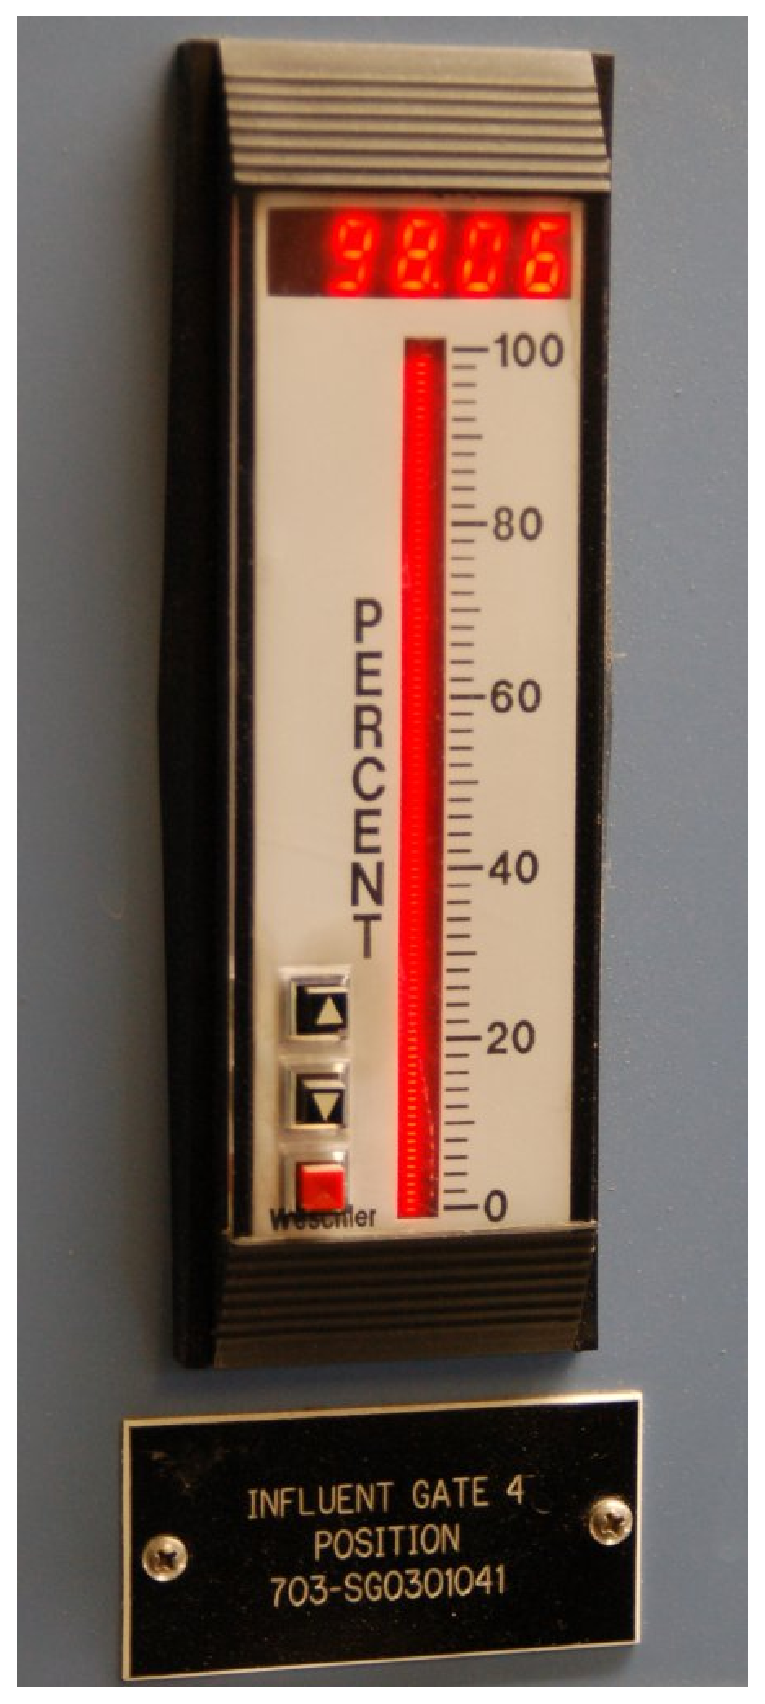
\includegraphics[height=4in]{intro_26.eps}$$

This particular indicator shows the position of a flow-control gate in a wastewater treatment facility, both by numerical value (98.06\%) and by the height of a bargraph (very near full open -- 100\%).  It is directly wired in series with the same 4-20 milliamp current signal sent to the gate actuator.  \index{Weschler panel-mounted bargraph indicator}

\filbreak

A less sophisticated style of panel-mounted indicator shows only a numeric display, such as this unit shown here:  \index{Red Lion Controls panel-mounted indicator}

$$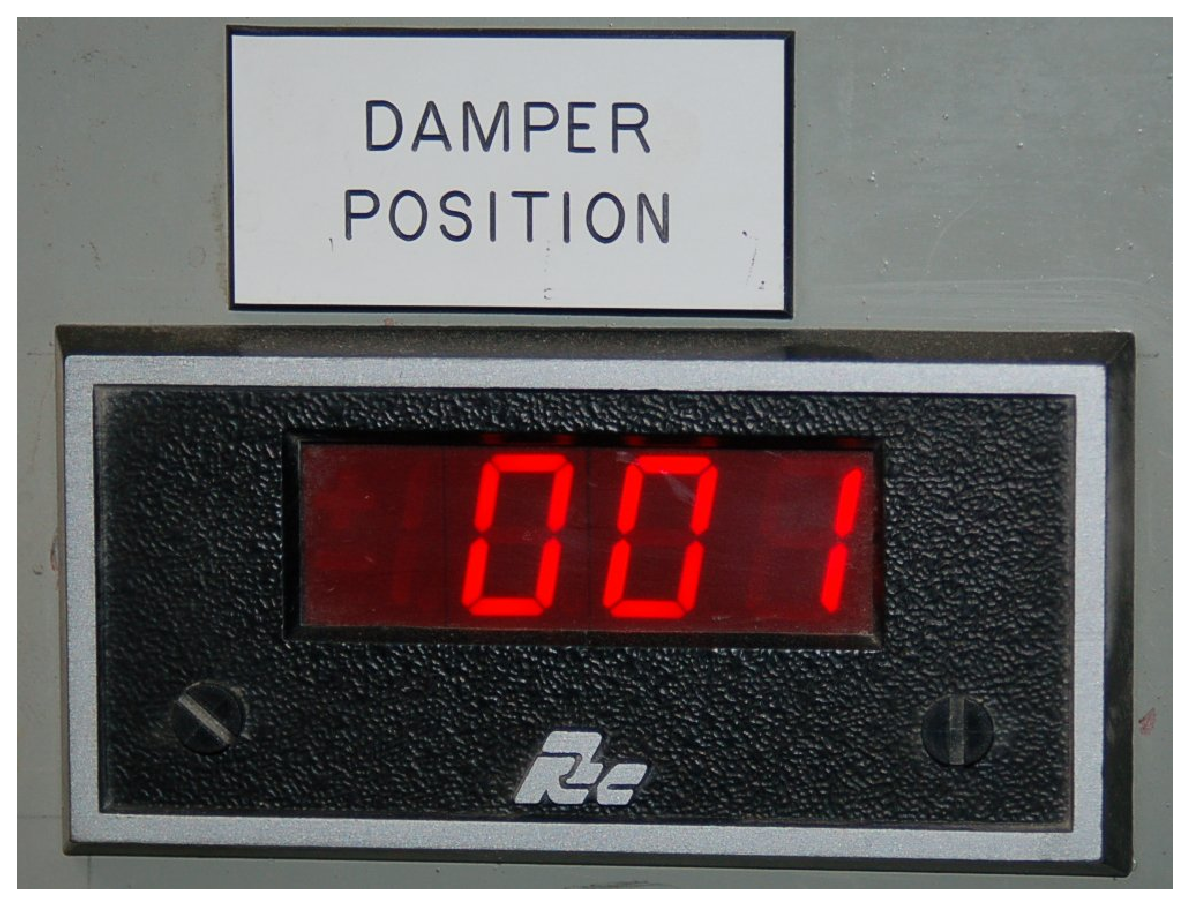
\includegraphics[width=4in]{intro_27.eps}$$

Indicators may also be used in ``field'' (process) areas to provide direct indication of measured variables if the transmitter device lacks a human-readable indicator of its own.  The following photograph shows a field-mounted indicator, operating directly from the electrical power available in the 4-20 mA loop.  The numerical display of this indicator uses LCD technology rather than red-glowing LEDs, in order to use less electrical power:  \index{Rosemount field-mounted indicator}

$$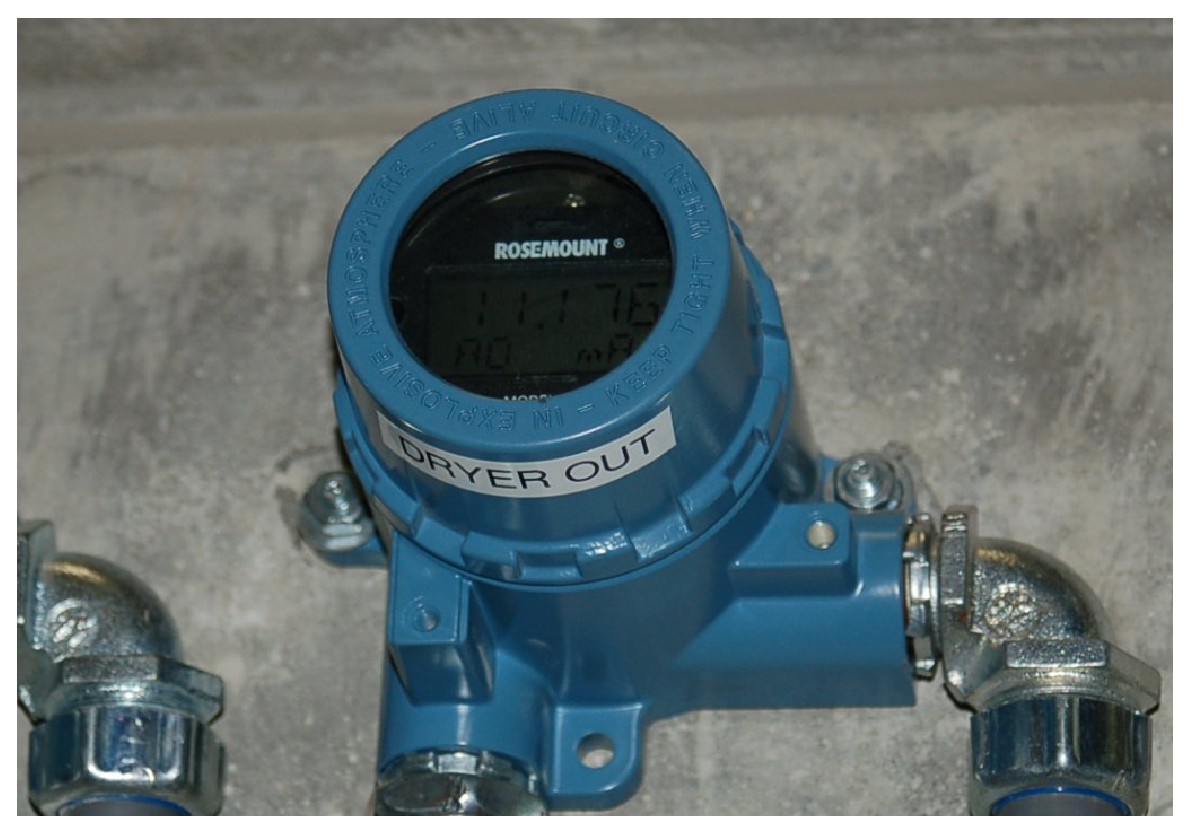
\includegraphics[width=4in]{intro_22.eps}$$





\filbreak
\subsection{Recorders}

Another common ``auxiliary'' instrument is the \textit{recorder} (sometimes specifically referred to as a \textit{chart recorder} or a \textit{trend recorder}), the purpose of which is to draw a graph of process variable(s) over time.  Recorders usually have indications built into them for showing the instantaneous value of the instrument signal(s) simultaneously with the historical values, and for this reason are usually designated as \textit{indicating} recorders.  A temperature indicating recorder for the nuclear reactor system shown previously would be designated as a ``TIR'' accordingly. \index{Recorder} \index{Chart recorder} \index{Trend recorder}

Paper chart recorders are a form of instrumentation with a long history.  The following image shows an illustration of a Bristol brand recording pressure gauge found on page 562 of \textit{Cassier's Magazine} volume 8, published in 1895.  Note the circular form of the paper chart, allowing the pen to draw a trace as the circular chart slowly spins.  A padlock on the front glass cover prevents tampering with the chart recording:  \index{Circular chart recorder}

$$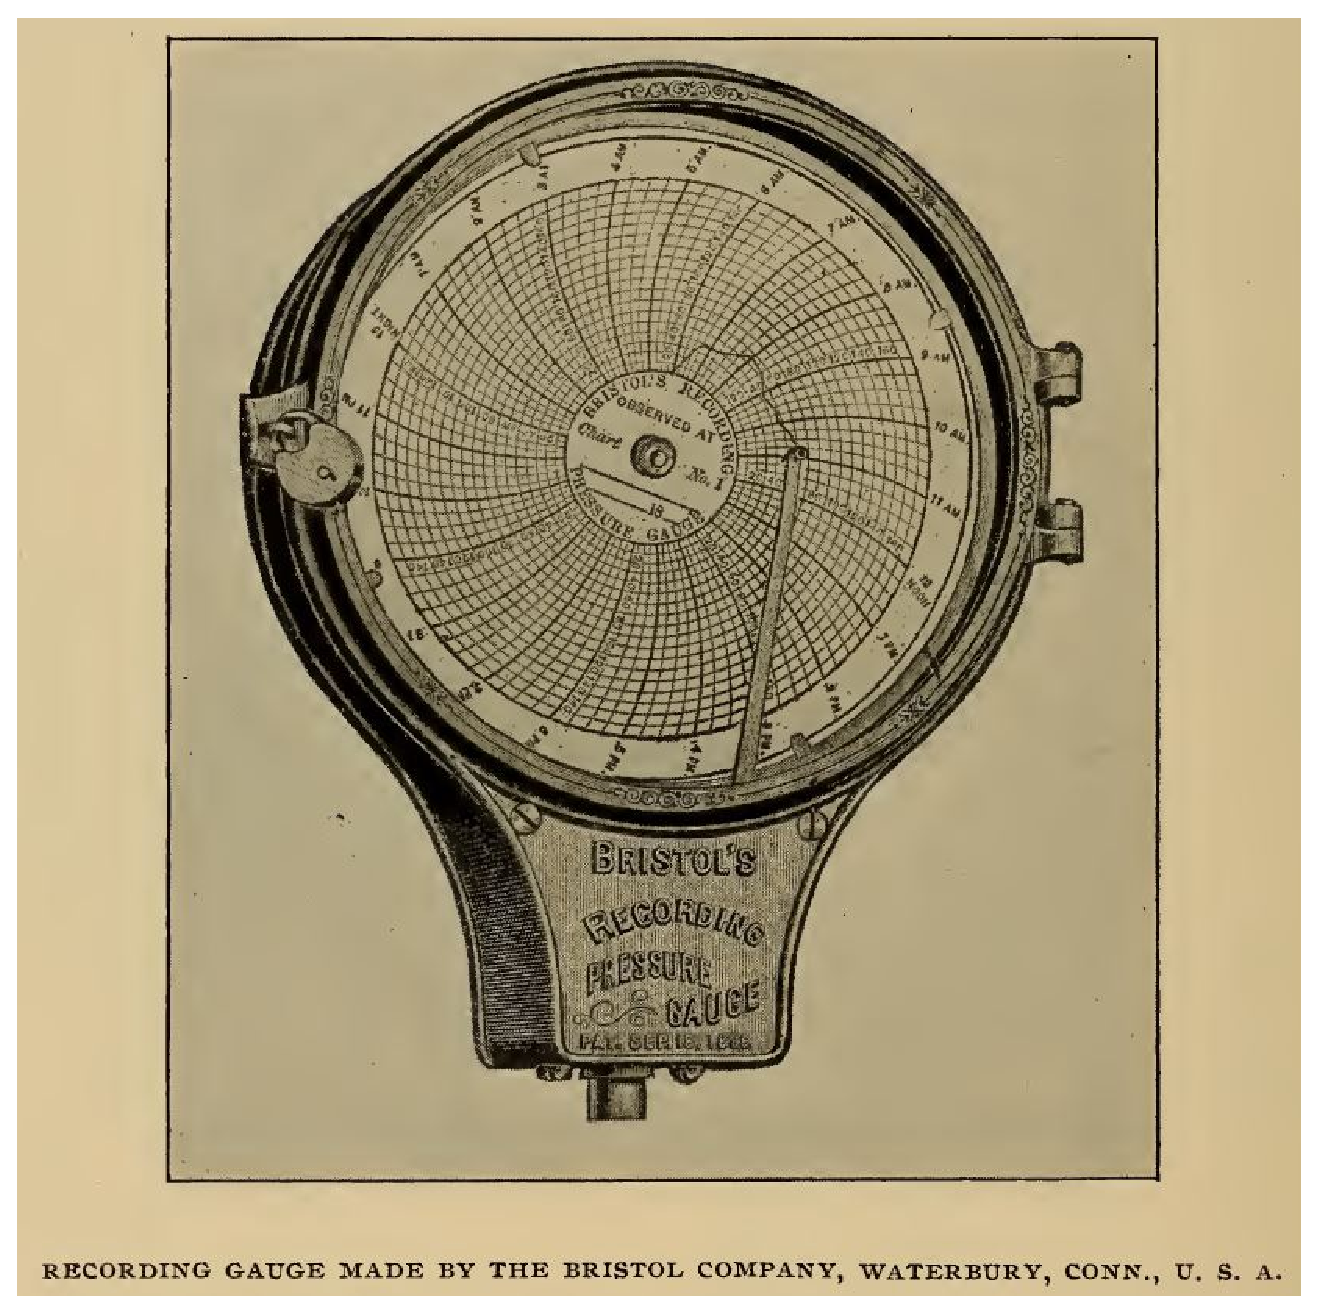
\includegraphics[height=4in]{intro_31.eps}$$

\filbreak

A typical chart from one of these recording devices is shown in this illustration, taken from page 563 of the same engineering periodical:

$$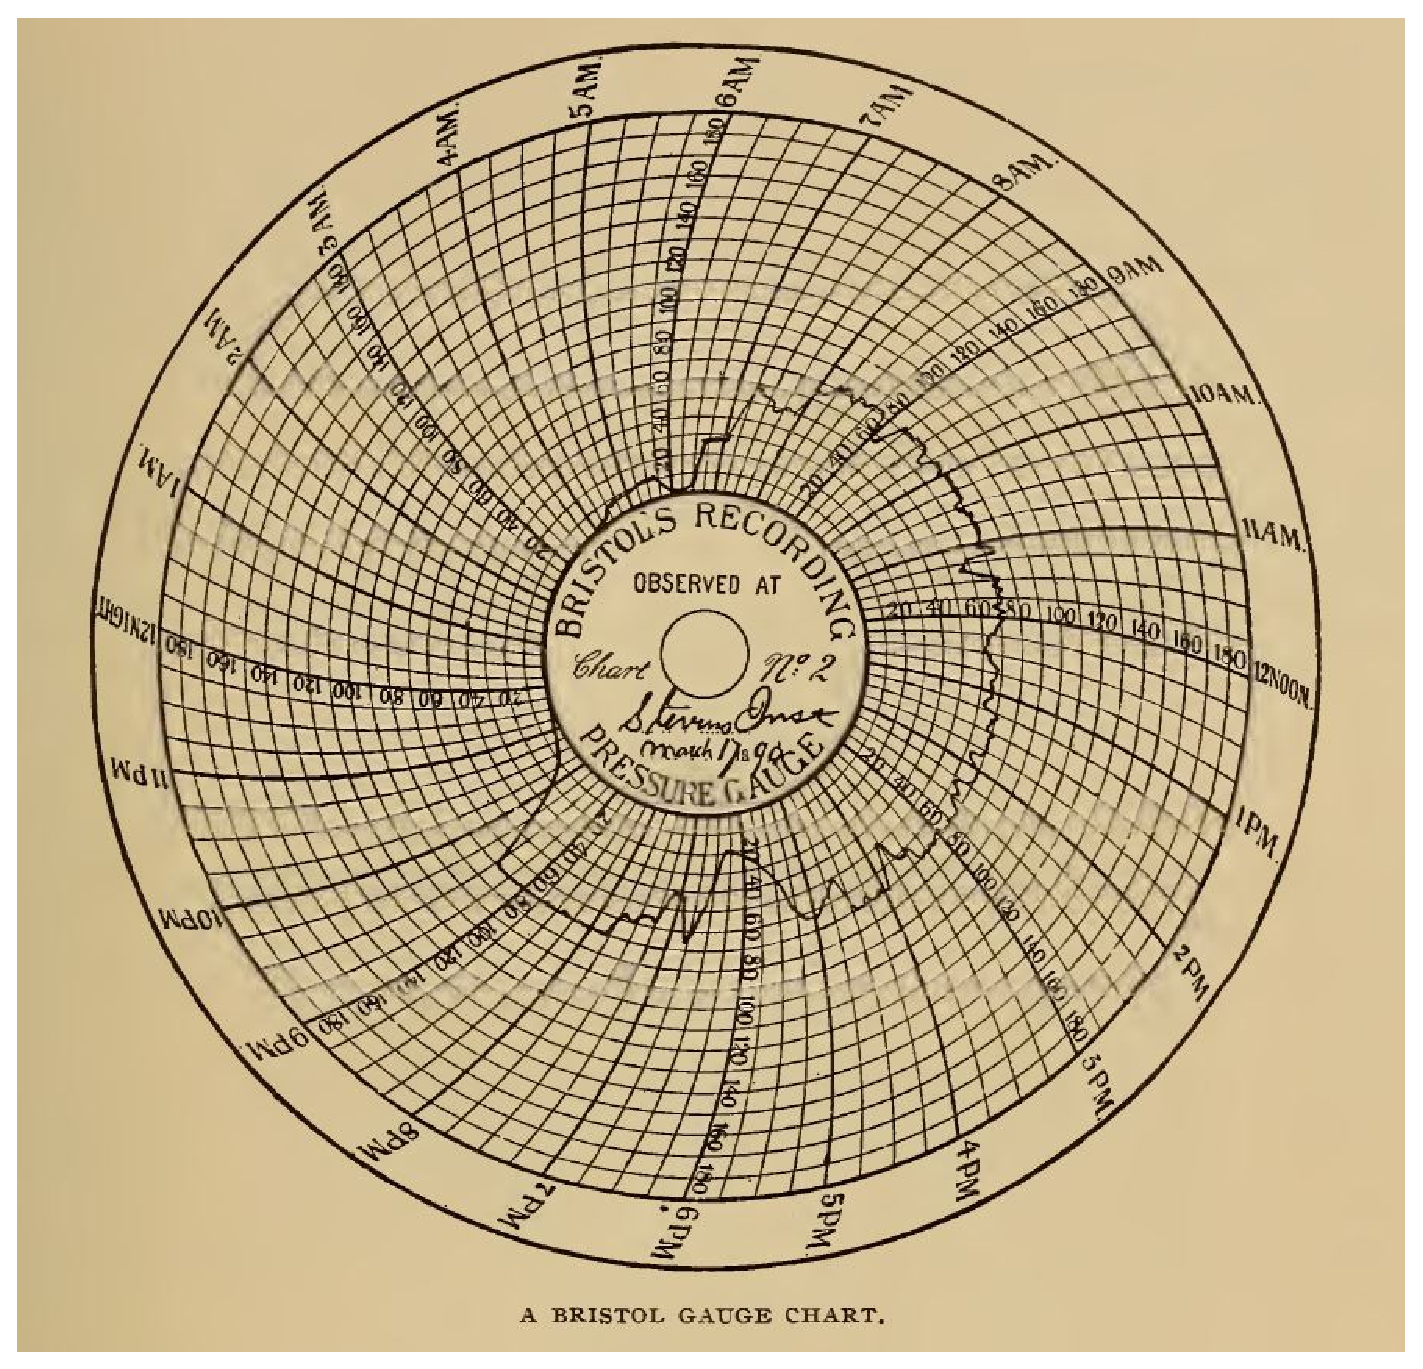
\includegraphics[width=6in]{intro_32.eps}$$

This particular recording is of a steam boiler's pressure over a 24-hour period, showing pressure build-up beginning at 4:00 AM and boiler shut-down at 9:30 PM.  This steam boiler's pressure appears to have been operated at approximately 70 PSI.  Dips and peaks in the trace reflect changes in steam demand as well as irregularities in the firing of the boiler's coal furnace.

\filbreak

Another design of paper chart recorder is the \textit{strip} style, using a long strip of paper between two spools (one to play out the paper and another to take it up).  Like the circular chart recorder design, the strip chart recorder also has a long history.  The following illustration from page 560 of the same \textit{Cassier's Magazine} volume:  \index{Strip chart recorder}

$$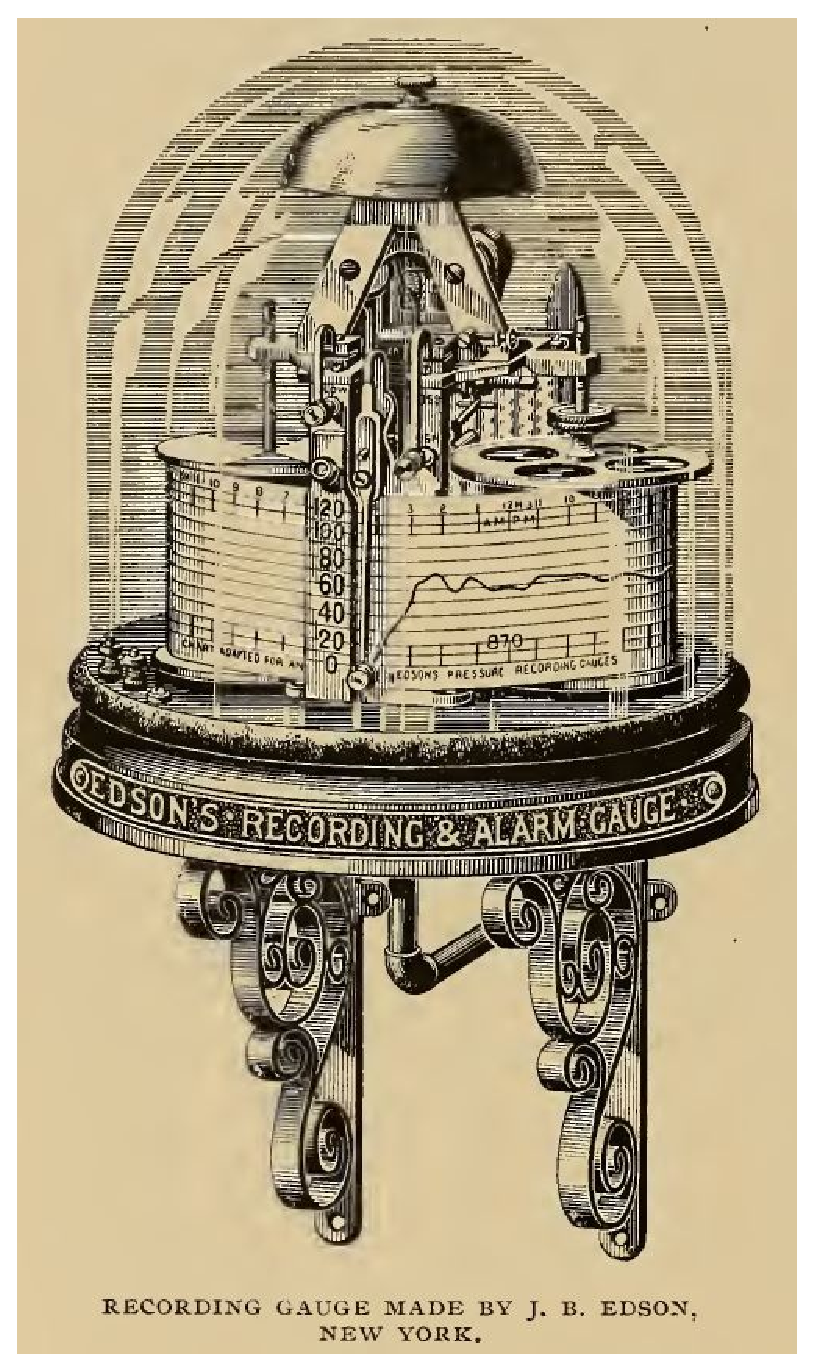
\includegraphics[height=3.5in]{intro_33.eps}$$

This next image shows a practical example of a strip chart's record for a city water supply company, taken from page 566 of the same periodical:  \index{Cassier's Magazine}

$$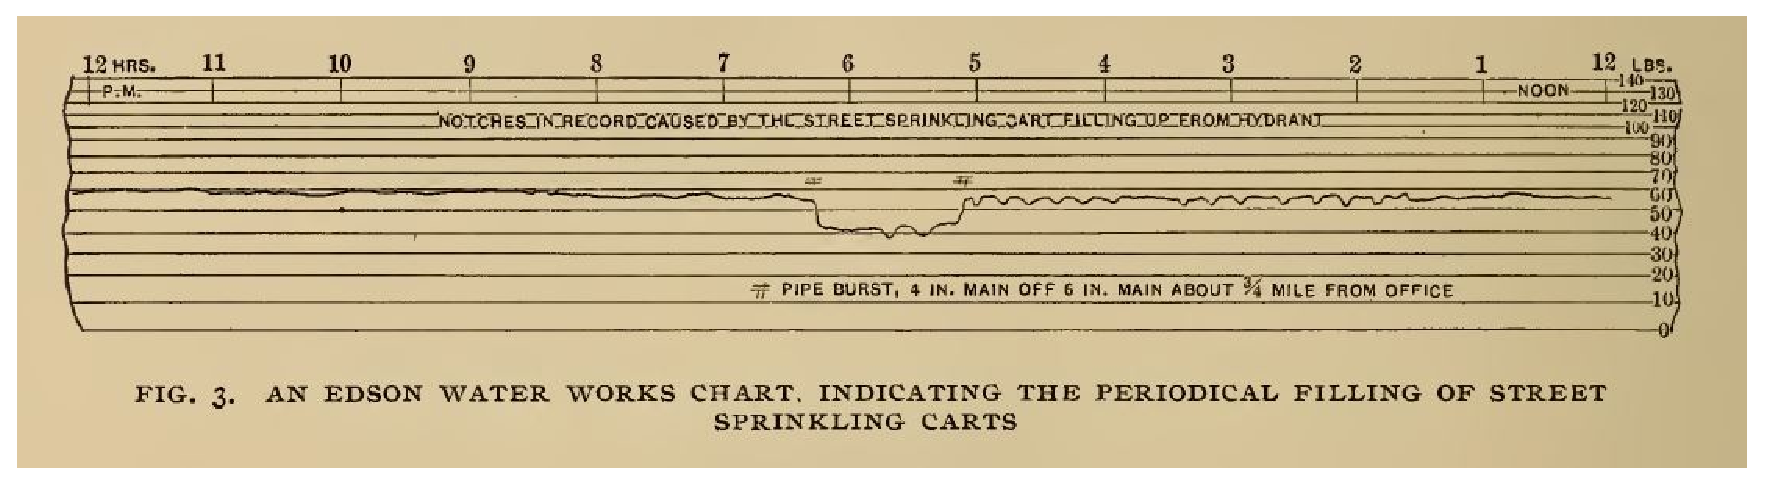
\includegraphics[width=5in]{intro_34.eps}$$

Several interesting details\footnote{\textit{Many} interesting points may be drawn from these two illustrations.  Regarding the strip chart recording instrument itself, it is worth noting the ornate design of the metal frame (quite typical of machinery design from that era), the attractive glass dome used to shield the chart and mechanism from the environment, and the intricate mechanism used to drive the strip chart and move the pen.  Unlike a circular chart, the length of a strip chart is limited only by the diameter of the paper roll, and may be made long enough to record many days' worth of pressure measurements.  The label seen on the front of this instrument (``Edson's Recording and Alarm Gauge'') tells us this instrument has the ability to alert a human operator of abnormal conditions, and a close inspection of the mechanism reveals a bell on the top which presumably rings under alarm conditions.  Regarding the strip chart record, note the ``compressed'' scale, whereby successive divisions of the vertical scale become closer in spacing, reflecting some inherent nonlinearity of the pressure-sensing mechanism.} may be seen on this particular recording, including pressure fluctuations caused by periodic draws of water from a fire hydrant to fill street carts used to spray the city's dirt roads with water to minimize dust.  Pressure drop caused by a burst 4-inch water pipe is also seen on this recording, between 5:00 PM and 6:15 PM.

\filbreak

Both circular and strip chart recorder designs survive to this day.  Two circular chart recorders are shown in the following photograph, used to record temperatures at a powdered milk processing facility:  \index{Circular chart recorder}

$$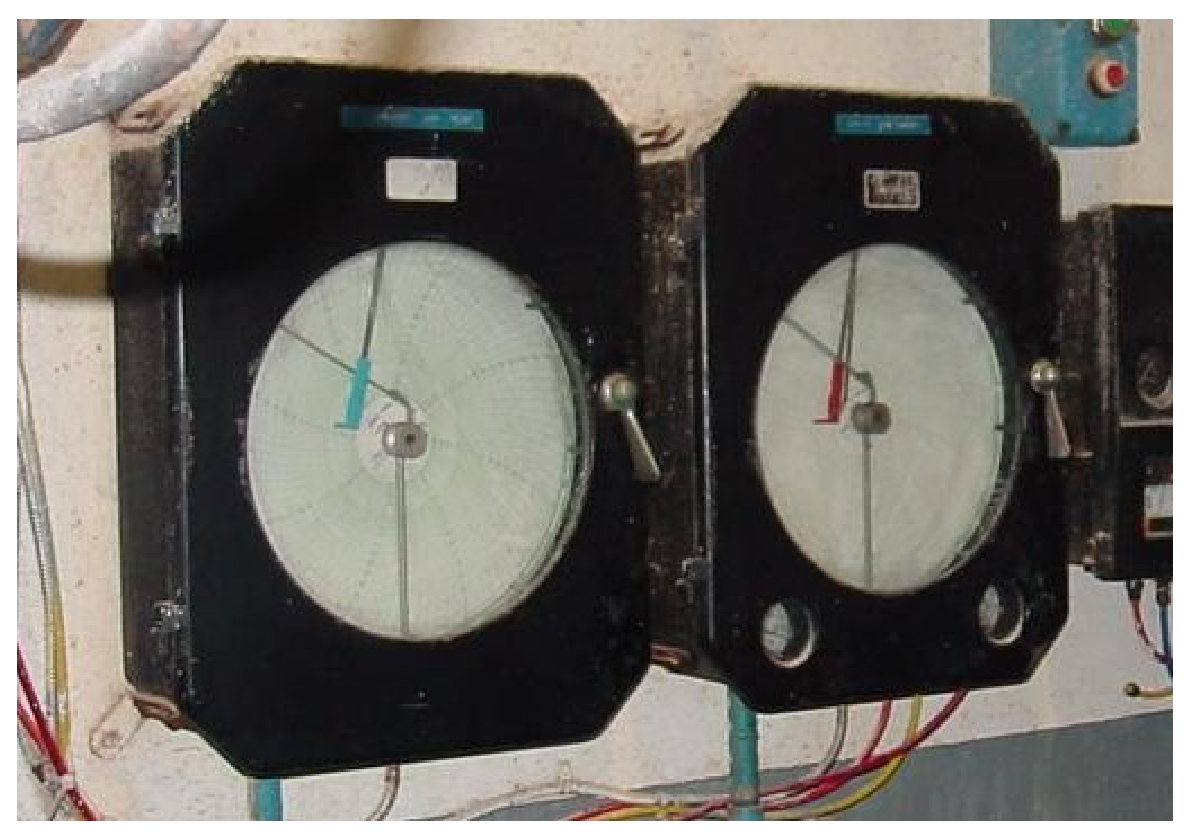
\includegraphics[width=4in]{intro_19.eps}$$

Two more chart recorders appear in the next photograph, a strip chart recorder on the right and a \textit{paperless} chart recorder on the left.  The strip chart recorder uses a scroll of paper drawn slowly past one or more lateral-moving pens, while the paperless recorder does away with paper entirely by plotting graphic trend lines on a computer screen:  \index{Paperless chart recorder}

$$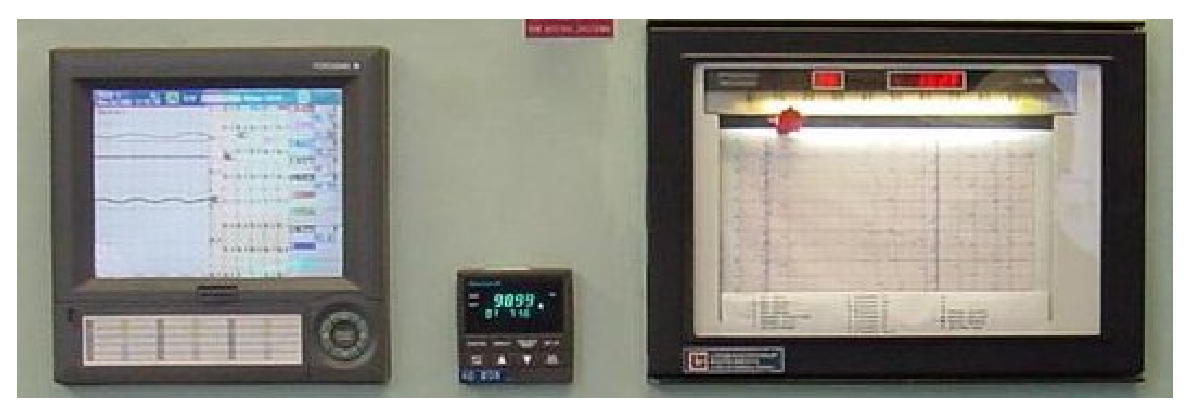
\includegraphics[width=4in]{intro_20.eps}$$

\filbreak

Recorders are extremely helpful for troubleshooting process control problems.  This is especially true when the recorder is configured to record not just the process variable, but also the controller's setpoint and output variables as well.  Here is an example of a typical ``trend'' showing the relationship between process variable, setpoint, and controller output in automatic mode, as graphed by a recorder:

$$\includegraphics{intro_05.eps}$$

Here, the setpoint (SP) appears as a perfectly straight red line, the process variable as a slightly erratic blue line, and the controller output as a moderately erratic purple line.  We can see from this trend that the controller is doing exactly what it should: holding the process variable value close to setpoint, manipulating the final control element as far as necessary to do so.  The chaotic appearance of the output signal is not really a problem, contrary to most peoples' first impression.  The fact that the process variable never deviates significantly from the setpoint tells us the control system is operating quite well.  What accounts for the erratic controller output, then?  The answer to this question is any factor requiring the controller to change its output in order to maintain the process variable at setpoint.  Variations in process load would account for this: as other variables in the process change over time, the controller is forced to compensate for these variations in order to ensure the process variable does not drift from setpoint.  Referencing our previous example of a steam boiler water level control system, one of these influencing variables is steam demand.  If this trend shows the steam drum water level (PV) and feedwater valve position (Output), variations in the controller's output signal could be indicative of steam demand rising and falling, the controller modulating water flow into the boiler to properly compensate for this load and maintain a fairly constant steam drum water level.  A wildly-fluctuating output signal \textit{may} indicate a problem somewhere else in the process (placing undue demands on the control system), but there is certainly no problem with the control system itself: it is doing its job perfectly well.

\vskip 10pt

Recorders become powerful diagnostic tools when coupled with the controller's manual control mode.  By placing a controller in ``manual'' mode and allowing direct human control over the final control element (valve, motor, heater), we can tell a lot about a process.  Here is an example of a trend recording for a process in manual mode, where the process variable response is seen graphed in relation to the controller output as that output is increased and decreased in steps:

$$\includegraphics{intro_06.eps}$$

Notice the time delay between when the output signal is ``stepped'' to a new value and when the process variable responds to the change.  This delay is called \textit{dead time}, and it is generally detrimental to control system performance.  Imagine trying to steer an automobile whose front wheels respond to your input at the steering wheel only after a 5-second delay!  This would be a very challenging car to drive.  The same problem plagues any industrial control system with a time lag between the final control element and the transmitter.  Typical causes of this problem include \textit{transport delay} (where there is a physical delay resulting from transit time of a process medium from the point of control to the point of measurement) and mechanical problems in the final control element.  \index{Dead time}  \index{Transport delay}

\filbreak

This next example shows another type of problem revealed by a trend recording during manual-mode testing:

$$\includegraphics{intro_07.eps}$$

Here, we see the process quickly responding to all step-changes in controller output except for those involving a change in direction.  This problem is usually caused by mechanical friction in the final control element (e.g. ``sticky'' valve stem packing in a pneumatically-actuated control valve), and is analogous to ``loose'' steering in an automobile, where the driver must turn the steering wheel a little bit extra after reversing steering direction.  Anyone who has ever driven an old farm tractor knows what this phenomenon is like, and how it detrimentally affects one's ability to steer the tractor in a straight line.

\vskip 10pt

Sometimes it becomes useful to temporarily place a recorder into an instrumentation system for diagnostic purposes.  On the simplest level, this might consist of a digital multimeter (DMM) connected to measure signal voltage or current, with its ``minimum/maximum'' capture mode engaged.  On a more complex level, this might be a personal computer running data graphing software, connected to the instrumentation circuit through a data acquisition (DAQ) module converting the circuit's analog voltage or current signals into digital values readable by the computer.  \index{Digital multimeter} \index{DMM}   \index{DAQ}  \index{Data acquisition module}






\filbreak
\subsection{Process switches and alarms}

Another type of instrument commonly seen in measurement and control systems is the \textit{process switch}.  The purpose of a switch is to turn on and off with varying process conditions.  Usually, switches are used to activate alarms to alert human operators to take special action.  In other situations, switches are directly used as control devices.  

\filbreak

The following P\&ID of a compressed air control system shows both uses of process switches: \index{Process switch} \index{Switch, process}

$$\includegraphics{intro_08.eps}$$

The ``PSH'' (\textit{pressure switch, high}) activates when the air pressure inside the vessel reaches its high control point.  The ``PSL'' (\textit{pressure switch, low}) activates when the air pressure inside the vessel drops down to its low control point.  Both switches feed discrete (on/off) electrical signals to a logic control device (symbolized by the diamond) which then controls the starting and stopping of the electric motor-driven air compressor.  

Another switch in this system labeled ``PSHH'' (\textit{pressure switch, high-high}) activates only if the air pressure inside the vessel exceeds a level beyond the high shut-off point of the high pressure control switch (PSH).  If this switch activates, something has gone wrong with the compressor control system, and the high pressure alarm (PAH, or \textit{pressure alarm, high}) activates to notify a human operator.

All three switches in this air compressor control system are directly actuated by the air pressure in the vessel: in other words, these are direct \textit{process-sensing} switches.  It is possible, however, to build switch devices that interpret standardized instrumentation signals such as 3 to 15 PSI (pneumatic) or 4 to 20 milliamps (analog electronic), allowing us to build on/off control systems and alarms for \textit{any} type of process variable measurable with a transmitter.  

\filbreak

For example, the chlorine wastewater disinfection system shown earlier may be equipped with a couple of electronic alarm switches to alert an operator if the chlorine concentration ever exceeds pre-determined high or low limits:

$$\includegraphics{intro_10.eps}$$

The labels ``AAL'' and ``AAH'' refer to \textit{analytical alarm low} and \textit{analytical alarm high}, respectively.  Note how the diagram shows these two alarm units connected to the electronic (4-20 mA) signal output by the chlorine analyzer (AT).  This tells us the AAL and AAH alarm units are really just electronic circuits, alarming if the analytical transmitter's 4-20 mA analog signal falls below (AAL) or exceeds (AAH) certain pre-set limits.  As such, the AAL and AAH alarms do not \textit{directly} sense the chlorine concentration in the water, but rather \textit{indirectly} sense it by monitoring the chlorine analyzer's 4-20 milliamp output signal.

Since both alarms work off the 4 to 20 milliamp electronic signal output by the chlorine analytical transmitter (AT) rather than directly sensing the process, their construction is greatly simplified.  If these were process-sensing switches, each one would have to be equipped with the analytical capability of directly sensing chlorine concentration in water.  In other words, each switch would have to be its own self-contained chlorine concentration analyzer, with all the attendant complexity.

\filbreak

An example of an electronic alarm module (triggered by a 4-20 mA current signal coming from a transmitter) is the Moore Industries model SPA (``Site Programmable Alarm''), shown here:  \index{Moore Industries model SPA alarm module}

$$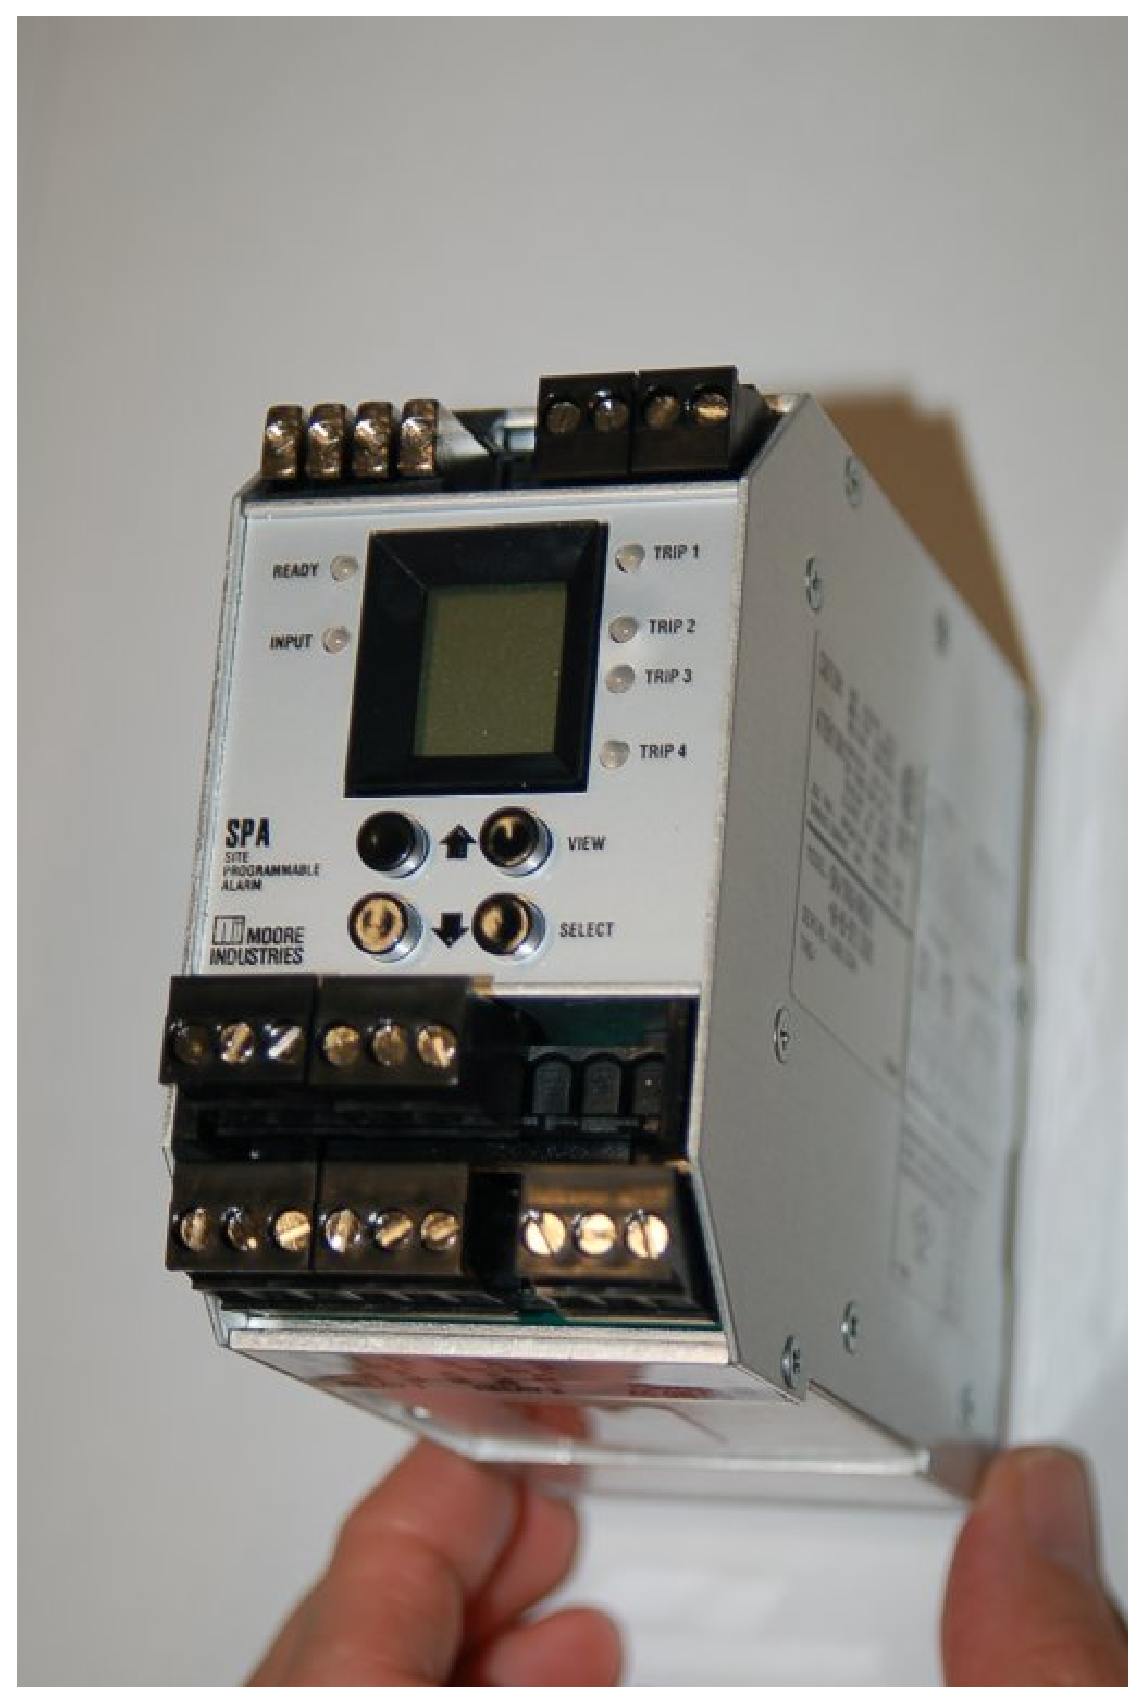
\includegraphics[width=3in]{intro_21.eps}$$

In addition to providing alarm capability, this SPA module also provides a digital display (a small LCD screen) to show the analog signal value for operational or diagnostic purposes.

Like all current-operated alarm modules, the Moore Industries SPA may be configured to ``trip'' electrical contacts when the current signal reaches a variety of different programmed thresholds.  Some of the alarm types provided by this unit include high process, low process, out-of-range, and high rate-of-change.

\filbreak

In a similar manner, we may add pressure-actuated process alarm switches to pneumatic (3-15 PSI) signal lines coming from pneumatic transmitters to add alarm capability to a system designed for continuous measurement.  For example, if high- and low-alarm capability were desired for the steam drum water level process described earlier in this chapter, one could add a pair of pressure-actuated switches to the pneumatic level transmitter's 3-15 PSI output signal line:

$$\includegraphics{intro_28.eps}$$

These two pressure-actuated switches serve as \textit{water level} alarms, because the air pressure signal actuating them comes from the pneumatic \textit{level} transmitter, which outputs an air pressure signal in direct proportion to water level in the boiler's steam drum.  Even though the physical stimulus actuating each switch is an air \textit{pressure}, the switches still serve the purpose of liquid \textit{level} alarm signaling because that air pressure is an analogue (representation) of water level in the steam drum.  In other words, these two alarm switches (LSL and LSH) \textit{indirectly} sense water level by monitoring the pneumatic signal pressure output by the level transmitter (LT).

\filbreak

The alternative to pressure-actuated water level alarm switches would be independent level-sensing switches attached directly to the steam drum, each switch equipped with its own means\footnote{These might be float-driven switches, where each switch is mechanically actuated by the buoyancy of a hollow metal float resting on the surface of the water.  Another technology uses metal electrodes inserted into the water from above, sensing water level by electrical conductivity: when the water level reaches the probe's tip, an electrical circuit is closed.  For more information on liquid level switches, refer to section \ref{level_switch} beginning on page \pageref{level_switch}.} of directly sensing water level:

$$\includegraphics{intro_29.eps}$$

\vskip 10pt

It should be mentioned that the choice between using process alarm switches directly actuated by the process versus alarm switches actuated by a transmitter's analog signal is not arbitrary.  In the system where the two alarm switches actuate from the transmitter's 3-15 PSI output signal, the integrity of the water level control \textit{and} that of the high- and low-level alarms all depend on the proper function of one transmitter.  If that one transmitter were to fail, all three system functions would be compromised.  This elevates the importance of a single instrument, which is generally not desirable from the perspective of reliability and process safety.  In the system where each level alarm switch independently senses steam drum water level, one device may fail without compromising either of the other two functions.  This independence is desirable because it greatly reduces the probability of ``common-cause'' failures, where a single fault disables multiple system functions.  The final determination should be based on a rigorous analysis of device versus system reliability, which is typically the task of a process engineer.

\filbreak

Process alarm switches may be used to trigger a special type of indicator device known as an \textit{annunciator}.  An annunciator is an array of indicator lights and associated circuitry designed to secure a human operator's attention\footnote{D.A. Strobhar, writing in \textit{The Instrument Engineers' Handbook} on the subject of alarm management, keenly observes that alarms are the only form of instrument ``whose sole purpose is to alter the operator's behavior.''  Other instrument devices work to control the process, but only alarms work to \textit{control the human operator}.} by blinking and sounding an audible buzzer when a process switch actuates into an abnormal state.  The alarm state may be then ``acknowledged'' by an operator pushing a button, causing the alarm light to remain on (solid) rather than blink, and silencing the buzzer.  The indicator light does not turn off until the actual alarm condition (the process switch) has returned to its regular state.  \index{Annunciator}  \index{Alarm, annunciator}

This photograph shows an annunciator located on a control panel for a large engine-driven pump.  Each white plastic square with writing on it is a translucent pane covering a small light bulb.  When an alarm condition occurs, the respective light bulb flashes, causing the translucent white plastic to glow, highlighting to the operator which alarm is active:

$$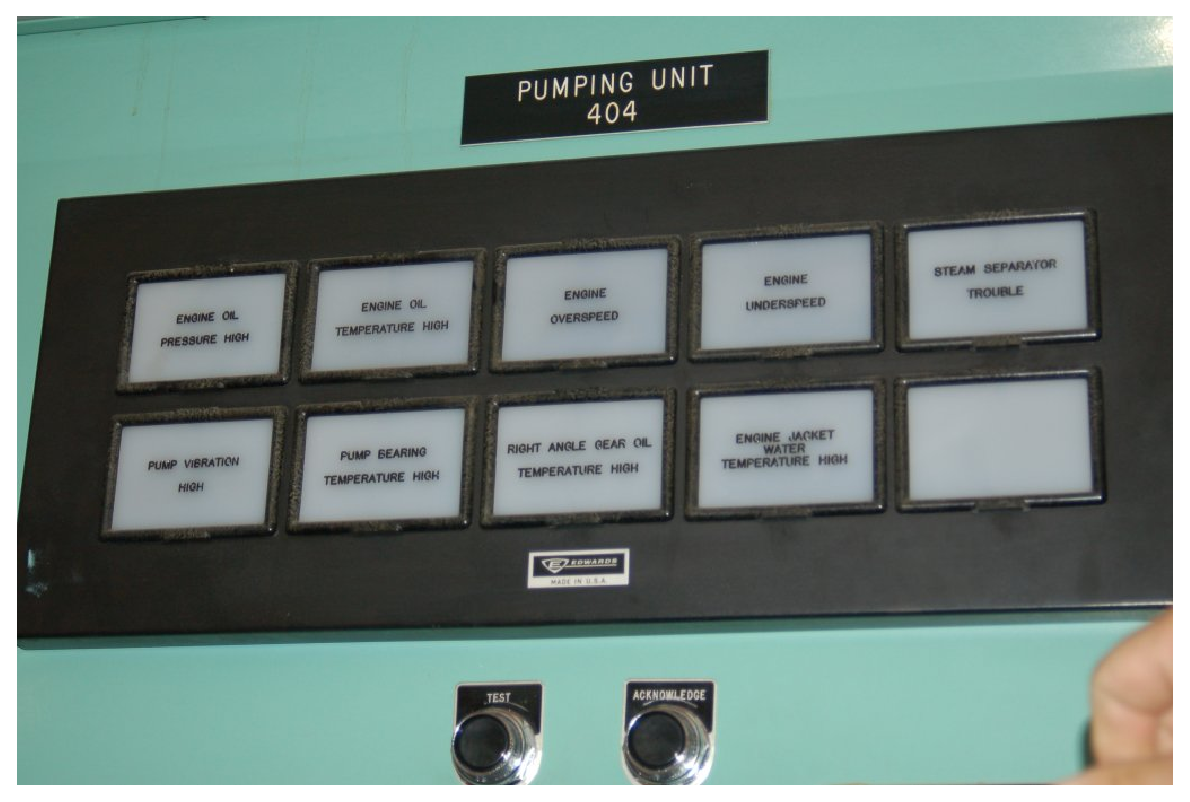
\includegraphics[width=5in]{intro_23.eps}$$

Note the two pushbutton switches below labeled ``Test'' and ``Acknowledge.''  Pressing the ``Acknowledge'' button will silence the audible buzzer and also turn any blinking alarm light into a steady (solid) alarm light until the alarm condition clears, at which time the light turns off completely.  Pressing the ``Test'' button turns all alarm lights on, to ensure all light bulbs are still functional.

\filbreak

Opening the front panel of this annunciator reveals modular relay units controlling the blinking and acknowledgment latch functions, one for each alarm light:

$$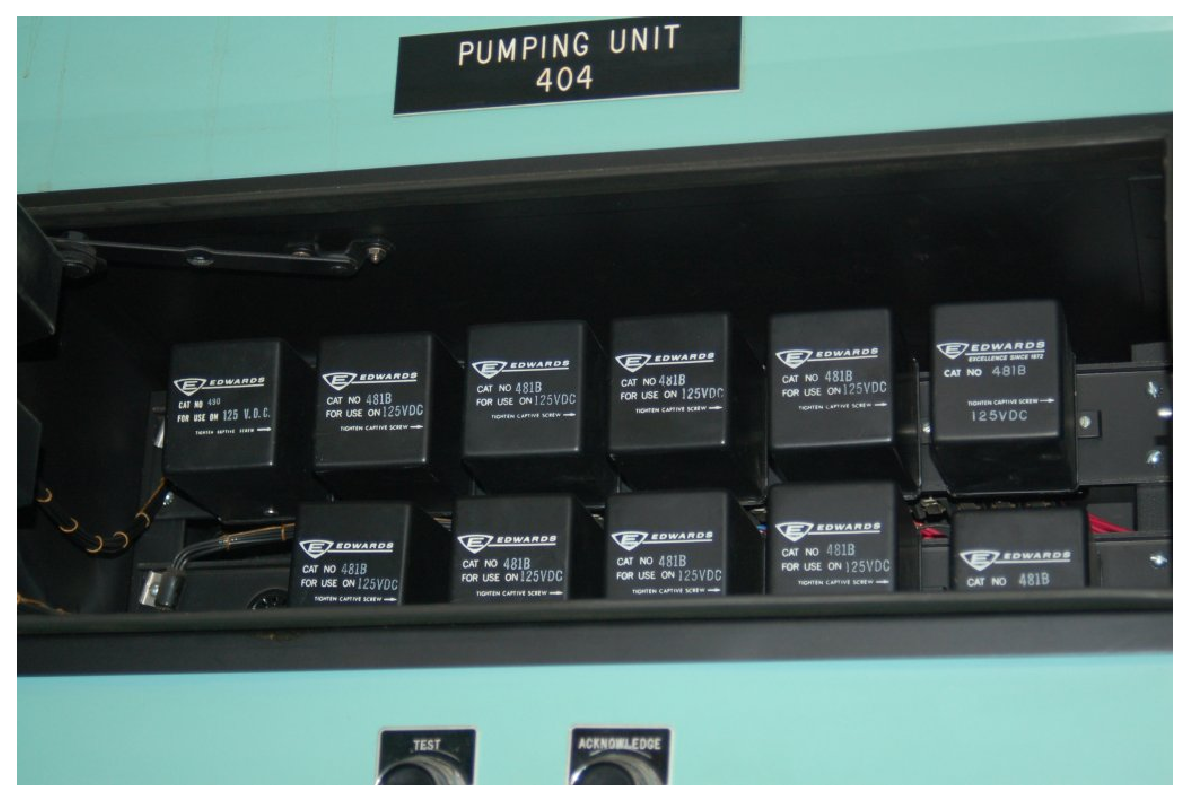
\includegraphics[width=5in]{intro_24.eps}$$

This modular design allows each alarm channel to be serviced without necessarily interrupting the function of the other channels in the annunciator panel.

\filbreak

A simple logic gate circuit illustrates the acknowledgment latching feature (here implemented by an S-R latch circuit) common to all process alarm annunciators:

$$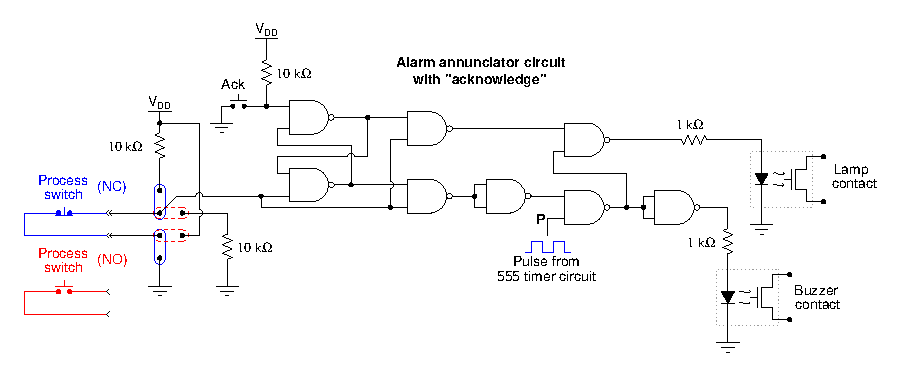
\includegraphics{intro_25.eps}$$

Panel-mounted annunciators are becoming a thing of the past, as computer-based alarm displays replace them with advanced capabilities such as time logging, first-event\footnote{When a complex machine or process with many shutdown sensors automatically shuts down, it may be difficult to discern after the fact \textit{which} shutdown device was responsible.  For instance, imagine an engine-powered generator automatically shutting down because one of the generator's ``trip'' sensors detected an under-voltage condition.  Once the engine shuts down, though, \textit{multiple} trip sensors will show abnormal conditions simply because the engine is not running anymore.  The oil pressure sensor is one example of this: once the engine shuts down, there will no longer be any oil pressure, thus causing that alarm to activate.  The under-voltage alarm falls into this category as well: once the engine shuts down, the generator will no longer be turning and therefore its output voltage \textit{must} be zero.  The problem for any human operator encountering the shut-down engine is that he or she cannot tell \textit{which} of these alarms was the initiating cause of the shutdown versus \textit{which} of these alarms simply activated after the fact once the engine shut off.  An annunciator panel showing both an under-voltage and a low oil pressure light does not tell us which event happened first to shut down the generator.  A ``first-event'' (sometimes called a ``first-out'') annunciator, however, shows which trip sensor was the \textit{first} to activate, thus revealing the initiating cause of the event.} recording, and multiple layers of acknowledgment/access.  Time logging is of particular importance in the process industries, as the sequence of events is often extremely important in investigations following an abnormal operating condition.  Knowing \textit{what happened, and exactly when it happened} is much more informative than simply knowing which alarms have tripped.





%\filbreak
%\section{Safety}

% ADD: Lock-out, tag-out (LOTO) procedures
% ADD: Photograph of lock station (Seattle WWTP tour photo)
% ADD: Photographs of danger tags
% ADD: Working with operations personnel to perform maintenance on operating instruments









\filbreak
\section{Summary}

Instrument technicians maintain the safe and efficient operation of industrial measurement and control systems.  This career requires a broad command of technical skill.  Instrumentation is more than just physics or chemistry or mathematics or electronics or mechanics or control theory or risk analysis or troubleshooting alone.  An instrument technician must know all these things to some degree, and more importantly how to synthesize and apply this knowledge to real applications.

The technical diversity of this profession is daunting.  Adding to this challenge is the continued adoption of new technologies.  The advent of new technologies, however, does not necessarily relegate legacy technologies to the scrap heap.  It is quite common to find state-of-the-art instruments in the very same facility as decades-old instruments; digital fieldbus networks installed alongside 3 to 15 PSI pneumatic signal tubes; microprocessor-based sensors mounted right next to old mercury tilt-switches.  Thus, the competent instrument technician must be comfortable working with both old and new technologies, understanding their merits, weaknesses, and especially their interactions.

This is why the most important skill for an instrument technician is the ability to teach oneself.  It is impossible to fully prepare for a career like this with any amount of preparatory schooling.  The profession is so broad and the responsibility so great, and the landscape so continuously subject to change, that life-long learning for the instrument technician is a matter of professional survival.  

\vskip 10pt

Perhaps the single greatest factor determining a person's ability to independently learn is their skill at \textit{reading}.  Being able to ``digest'' the written word is \textit{the} key to learning what is difficult or impractical to directly experience.  In an age where information is readily accessible, the skilled reader has the advantage of leveraging generations of experts in virtually any subject.  Best of all, reading is a skill anyone can master, and everyone should.

My advice to all those desiring to become self-directed learners is to build a library of reading material on subjects that interest you (hopefully, instrumentation is one of those subjects!), and then immerse yourself in those writings.  Feel free to ``mark up\footnote{A fun and informative essay to read on this subject is Mortimer Adler's \textit{How to Mark a Book}, widely disseminated on the Internet.  In it, Adler argues persuasively for the habit of annotating the books you read, and gives some practical tips for doing so.  He says reading a book should be a sort of \textit{conversation with the author} where the flow of information is not just from the author to you, but also from you to yourself as you question, consider, and even argue the author's points.}'' your books, or take notes in a separate location, so as to actively engage in your reading.  Try as much as possible to approach reading as though you were having a \textit{conversation} with the author: pose questions, challenge concepts and ideas, and do not stop doing so until you can clearly see what the author is trying to say.

I also advise \textit{writing} about what you learn, because explaining new ideas in your own words helps you consolidate the learning, and ``makes it your own'' in a way few other activities do.  You don't necessarily have to write your own book, but the act of expressing what you have learned is a powerful tool not only for building understanding, but also for revealing what you do not (yet) know.  A method I have used with great success is to imagine myself having to explain a new concept to a precocious child: someone with enough mental capacity to grasp the concept but lacking the necessary vocabulary and experience to grasp a sophisticated presentation of it.  This mental exercise forces you to explain things as simply as possible without error (because anyone can devise an explanation that is both simple and wrong!).  All teachers know the power of this technique: you never learn a subject as well as when you must teach it to someone else.









\filbreak
\section{Review of fundamental principles}

Shown here is a partial listing of principles applied in the subject matter of this chapter, given for the purpose of expanding the reader's view of this chapter's concepts and of their general inter-relationships with concepts elsewhere in the book.  Your abilities as a problem-solver and as a life-long learner will be greatly enhanced by mastering the applications of these principles to a wide variety of topics, the more varied the better.

\begin{itemize}
\item \textbf{Representative signal}: using a signaling medium such as compressed air, electric current, or voltage pulses to represent some range of measured variable.
\item \textbf{Common-cause failures}: when multiple functions in a system depend on a single element, failure of that element will cause all dependent functions to fail.  Relevant to design of process alarm switches.
\item \textbf{Negative feedback}: when the output of a system is degeneratively fed back to the input of that same system, the result is decreased (overall) gain and greater stability.  Relevant to loop controller action: in order for a control system to be stable, the feedback must be negative.
\end{itemize}







\filbreak
\section*{References}

% In alphabetical order!
% \noindent
% Lastname, Firstname MiddleI., \textit{Book Title}, Publisher, City, State, Year.
% \vskip 10pt
% \noindent
% Lastname, Firstname MiddleI., \textit{Book Title}, Publisher, City, State, Year.
% etc . . .

\noindent
Adler, Mortimer, ``How to Mark a Book'', \textit{The McGraw-Hill Reader}, McGraw-Hill Book Company, New York, NY, 1982.

\vskip 10pt

\noindent
Hague, Charles A. ``The Recording Gauge Applied to Water Pressure and Other Uses'', \textit{Cassier's Magazine} Volume 8, 1895.

\vskip 10pt

\noindent
Lipt\'ak, B\'ela G. et al., \textit{Instrument Engineers' Handbook -- Process Software and Digital Networks}, Third Edition, CRC Press, New York, NY, 2002.












%%%%%%%%%%%%%%%%%%%%%%%%%%%%%%%%%%%%%%%%%%%%%%%%%%%%

